\documentclass[12pt]{beamer}
\usepackage[T1]{fontenc}
\usepackage[utf8]{inputenc}
\usetheme[]{Honefoss}
\usepackage{hyperref}
\hypersetup{
    colorlinks=true,
    linkcolor=blue,
    filecolor=magenta,      
    urlcolor=cyan,
}

\urlstyle{same}

\title{Satellite Orbits in Python}
\author{Ingrid Fausk, Michael D\"ahnn, Ann-Silje Kirkvik}
\date{Sep 22, 2020}

\begin{document}
\frame{\titlepage}


\begin{frame}{Norwegian Mapping Authority - NMA}
\begin{itemize}
\item
  Geographical Information
\item
  Property Registry
\item
  Geodesy
\end{itemize}
\end{frame}


\begin{frame}{Geodesy}
The science of accurately measuring and understanding Earth's geometric shape, orientation in space and gravitational field, and how these properties change over time.
\end{frame}


\begin{frame}{Satellite Laser Ranging}
  \begin{tabular}{cl}
    &  \\
    \raisebox{-.5\height}{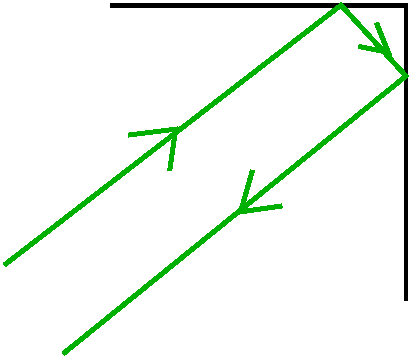
\includegraphics[width=0.2\textwidth]{figure/laser.eps}} & 
    \begin{minipage}[t]{0.6\columnwidth}{\it Retroreflectors} make sure that light is reflected back to its source\end{minipage}\\
    &  \\     
    \raisebox{-.5\height}{\includegraphics[width=0.2\textwidth]{figure/plotkin_-_beacon_explorer_a2.jpg}} & 
    \begin{minipage}[t]{0.6\columnwidth}Henry Plotkin with the first satellite equipped with retroreflectors, Beacon Explorer B, 1964. \end{minipage}\\
  \end{tabular}
\end{frame}


\begin{frame}{LAser GEOdynamics Satellite}
  \begin{columns}
    \column{0.6\textwidth}
      \begin{itemize}
        \item LAGEOS-1, 1976 (USA) 
        \item LAGEOS-2, 1992 (Italy)
        \item Weight: 400 kg
        \item Period: 220 min
        \item Height: 5800 km
        \item Diameter: 60 cm
        \item Life expectancy: 8.4 mill years 
      \end{itemize}
      
    \column{0.3\textwidth}
        \includegraphics[width=0.7\textwidth]{figure/lageos_1.jpg} \\Photo: NASA
  \end{columns}
  
\end{frame}


\begin{frame}{Our Ambitions in Laser Ranging}
  \vspace{0.7cm}
  \begin{columns}
    \column{0.45\textwidth}
      \includegraphics[width=0.95\textwidth]{figure/jordklode.eps}
    \column{0.45\textwidth}
      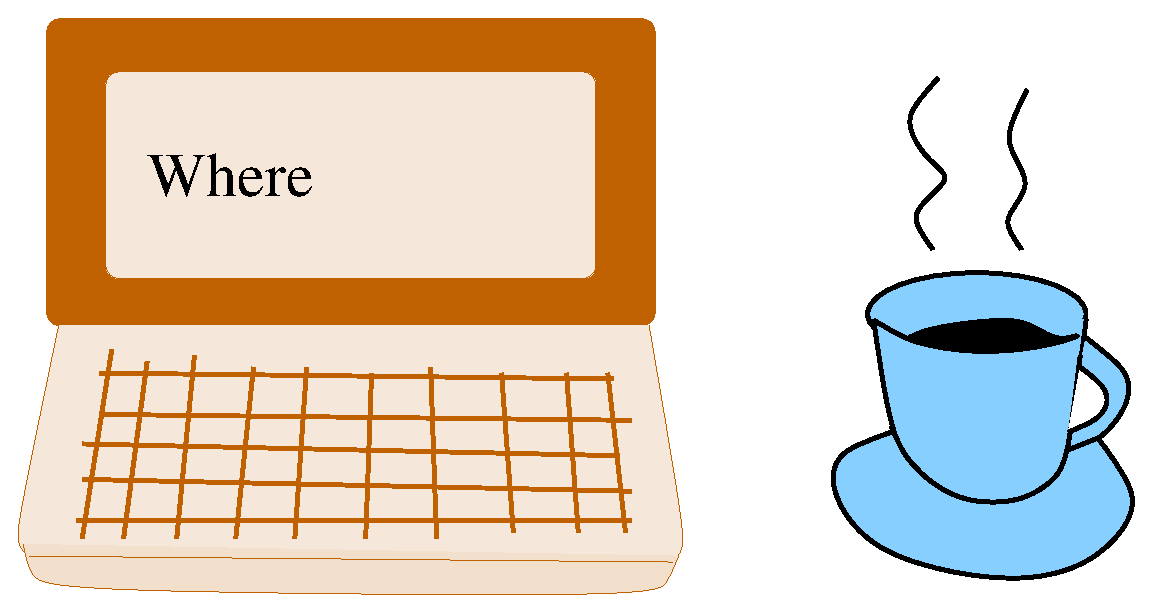
\includegraphics[width=0.95\textwidth]{figure/where.eps}
  \end{columns}
\end{frame}


\begin{frame}{Earth Observatory - Ny Ålesund}
 \begin{itemize}
     \item VLBI antennas
     \item In the future also laser ranging instrument
     \item Observe polar-orbiting satellites with good coverage
     \item $79 ^{\circ}$ North
 \end{itemize}\ \\ \ \\
 
 \includegraphics[]{figure/antennebilde.jpg}\ \\ 
  {\small Photo: Bjørn-Owe Holmberg}
\end{frame}


\begin{frame}{ITRF}
\framesubtitle{International Terrestrial Reference Frame}
  \begin{description}
    \item[Why?] To measure plate tectonics, ocean level, mass displacements etc. in reference to something
    \item[How?] Made with four geodetic techniques; GPS, VLBI, SLR and DORIS
    \item[When?] It is updated every few years, because the Earth is changing, and surveying techniques are changing
    \item[Last time:] ITRF2014
    \item[Next time:] ITRF2020
  \end{description}
\end{frame}


\begin{frame}{The Reference Frame}
  \begin{columns}
    \column{0.22\textwidth}\\ \ \\ \ \\
        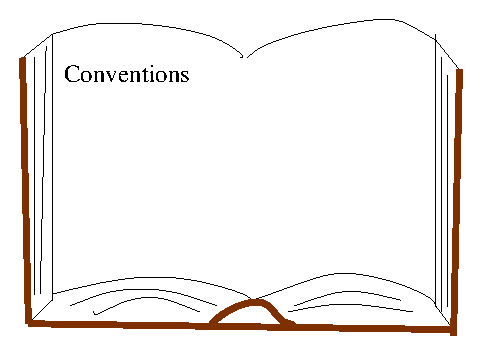
\includegraphics[width=0.95\textwidth]{figure/book.eps}\\ \ \ Rules
    \column{0.08\textwidth}\\ \ \\ 
      +  
    \column{0.22\textwidth}
        \includegraphics[width=0.95\textwidth]{figure/jordklode.eps}\\ Observations
    \column{0.08\textwidth}\\ \ \\ 
      =
    \column{0.26\textwidth}\\ \ \\ 
        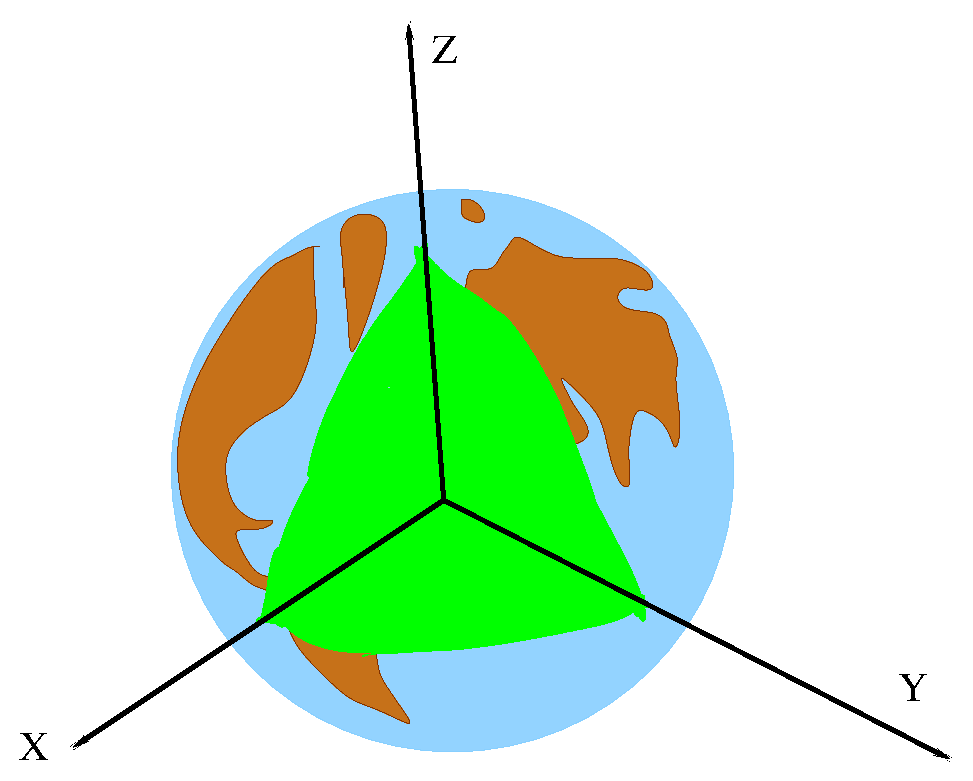
\includegraphics[width=0.97\textwidth]{figure/referanseramme.eps}\\ Referance Frame
  \end{columns}
\end{frame}


\begin{frame}{Earth Orientation Parameters}
  \framesubtitle{How celestial system is rotated w.r.t terrestrial system}
  \begin{center}
    \includegraphics[width=0.15\textwidth]{figure/eop_parameters.png}
    \\
    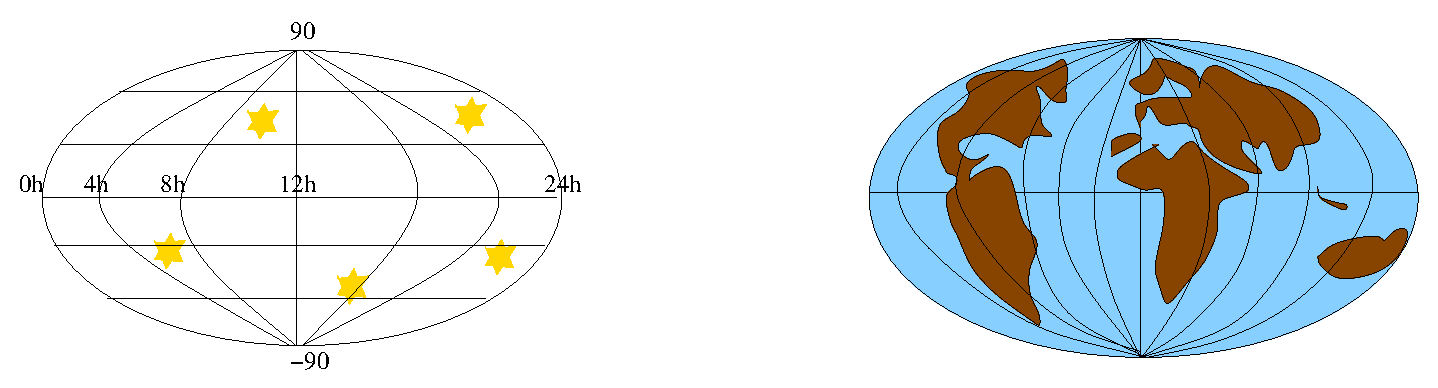
\includegraphics[width=0.8\textwidth]{figure/eop.eps}
  \end{center}
\end{frame}


\begin{frame}{Where}
\begin{itemize}
\item 
  \textit{Where} is a Python software package used for analyzing geodetic data from satellites and quasars
\item
  \textit{Where} is currently being developed at the Norwegian Mapping Authority (NMA)
\item
  \textit{Where} is an open source project, available on github \url{https://github.com/kartverket/where}
\end{itemize}
\end{frame}


\begin{frame}{Technology}

The \textit{Where} software is mainly being written in \emph{Python}
\begin{itemize}
\item
  Solid, flexible and fast libraries like \texttt{numpy},
  \texttt{matplotlib} and \texttt{scipy} are available
\item
  We use a \textbf{HDF5}-based format for storing data
\item
  Python has effective interfaces to \emph{C} and \emph{Fortran}
  code, and we can use external libraries directly
\end{itemize}
\end{frame}


\begin{frame}{Useful Features}
\begin{itemize}
\item
  Logging of events that occur while software runs. 
\item 
  Configuration files defines the details on how the analysis is done. Examples include what data is used, how to clean the data before analysis and which parameters to estimate.
\item 
  Dataset with time objects, position and velocity objects, including conversion routines. 
\end{itemize}
\end{frame}
 

\begin{frame}{There}

\textit{Where} is a command line tool, but the results can be inspected using the graphical tool called \textit{There}. A screenshot is shown below.

\begin{center}
  \includegraphics[height=0.6\textheight]{./figure/there.png}
\end{center}
\end{frame}


\begin{frame}{Using Where}
\begin{itemize}
\item 
  MIT Open Source License: Permissive, use \textit{Where} as you want
\item
  But please acknowledge us if you use \textit{Where}
\item 
  Get in touch if you are interested in \textit{Where}
\end{itemize}
\end{frame}


\begin{frame}{Three types of models}
  \begin{columns}
    \column{0.5\textwidth}
      \begin{figure}
        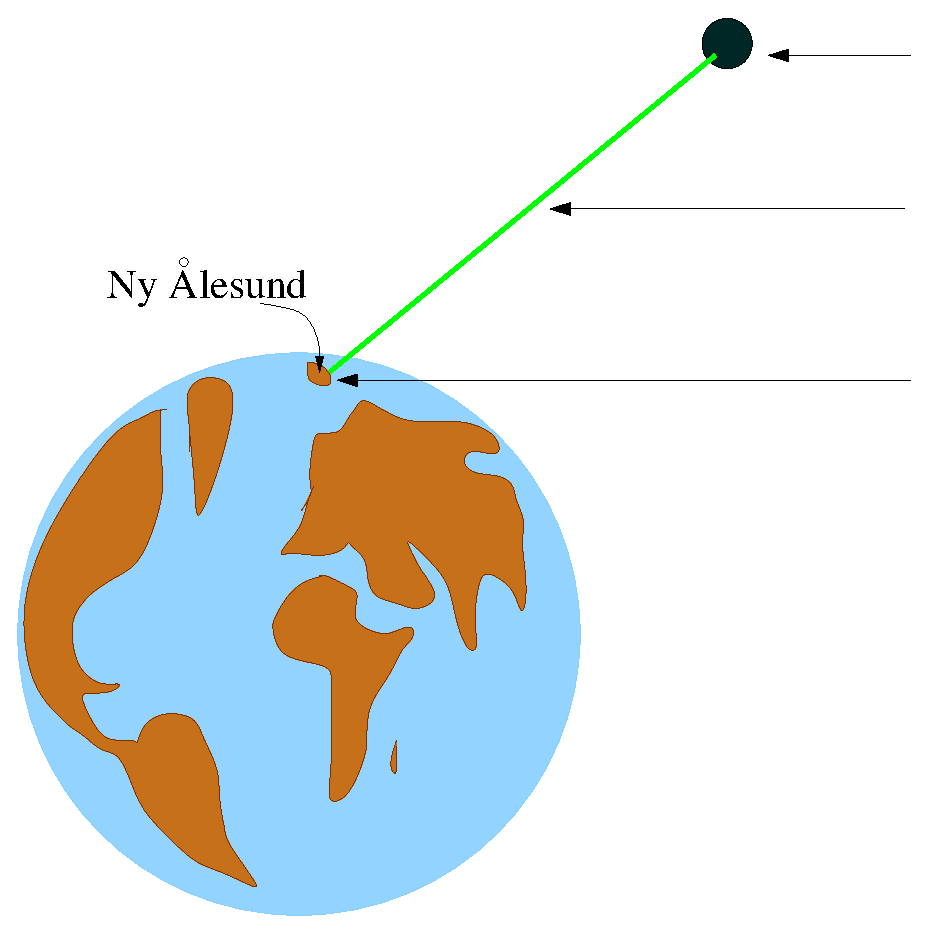
\includegraphics[width=0.95\textwidth]{figure/korreksjoner.eps}
      \end{figure}
    \column{0.45\textwidth}
        Models for satellitte orbit\vspace{0.4cm}
        Delay of signal\vspace{0.4cm} \\
        Station displacements\vspace{2.5cm}
  \end{columns}
\end{frame}


\begin{frame}{Forces acting on the Satellite}
\begin{itemize}
\item
  Gravity from Earth, Moon, Sun and planets
\item 
  Solar radiation pressure
\item 
  Solid earth tides and ocean tides
\item 
  Relativity
\end{itemize}
\end{frame}


\begin{frame}{Orbit determination 1}
\includegraphics[width=0.8\textwidth]{figure/orbit1.png} \\ Starting out with initial position and velocity
\end{frame}


\begin{frame}{Orbit determination 2}
\includegraphics[width=0.8\textwidth]{figure/orbit2.png} \\ Compute orbit from force models, this is the heavy part, using numerical integration
\end{frame}


\begin{frame}{Orbit determination 3}
\includegraphics[width=0.8\textwidth]{figure/orbit3.png} \\ Add some observations
\end{frame}


\begin{frame}{Orbit determination 4}
\includegraphics[width=0.8\textwidth]{figure/orbit4.png} \\ Estimate new initial position and velocity using least squares, and compute new orbit 
\end{frame}


\begin{frame}{Orbit determination problems}
  All models are implemented, but...
\begin{itemize}
\item 
  Orbit residuals are a few centimeters too large, so we are currently debugging the orbit models
\item
  The orbit determination is a bit slow, compared to similar fortran programs
\end{itemize}
\end{frame}

\end{document}

